\section{Data Analysis}

In this section, we present our results after the execution of sorting algorithms over the input files. We analyzed only two of the four dependent variables, which were \textit{percentage of the largest subarray size (\%LSS)} and \textit{percentage of unordered elements quantity (\%UEQ)}. These variables, because they are a percentage value, already were normalized (i.e., the same order of magnitude) related to dependent variable \textit{array size}.

\subsection{Exploratory Data Analysis (EDA)}

Firstly, we performed an analysis of the distribution of the dependent variables \%LSS and \%UEQ. To help in this task, we produced histograms, boxplot graphs, tables containing data about mean, median, standard deviation, and the minimum and maximum values.

The following Figures \ref{fig-histogram-lss-001-100}, \ref{fig-histogram-ueq-001-100} and \ref{fig-boxplots-001-100} illustrates examples of histograms and boxplot graphs for each combination of \textit{Algorithm X Probability of Failure X Array Size}. In each of those figures, the graphs were exhibited over the dependent variables \%LSS and \%UEQ.

\begin{figure}[H]
    \centering
     \begin{subfigure}{.5\textwidth}
     \centering
     \frame{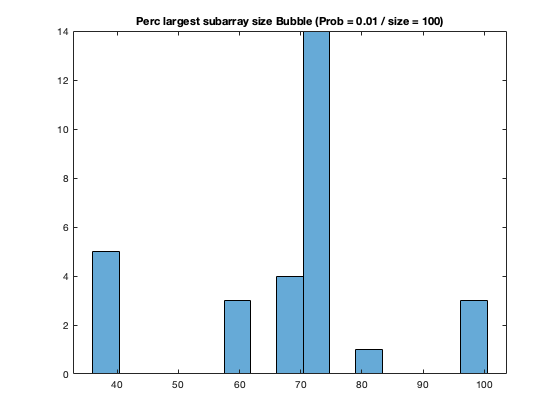
\includegraphics[scale=0.45]{figures/histogram_bubble_LSS_001_100.png}}
     \textsf{\caption[Histogram for Bubblesort.]{Histogram for Bubblesort.\label{fig-histogram-bubble-lss-001-100}}}
     \end{subfigure}%
     \begin{subfigure}{.5\textwidth}
     \centering
     \frame{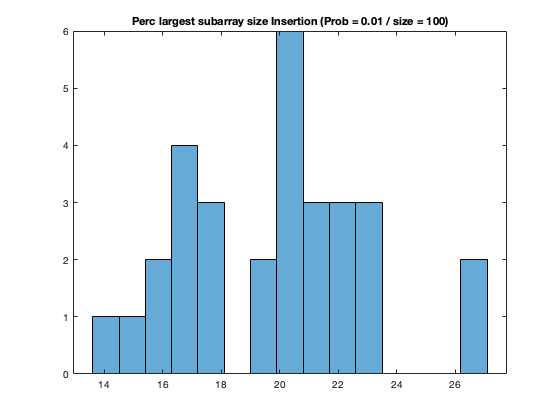
\includegraphics[scale=0.45]{figures/histogram_insertion_LSS_001_100.png}}
     \textsf{\caption[Histogram for Bubblesort.]{Histogram for Bubblesort.\label{fig-histogram-insertion-lss-001-100}}}
     \end{subfigure}
     \begin{subfigure}{.5\textwidth}
     \centering
     \frame{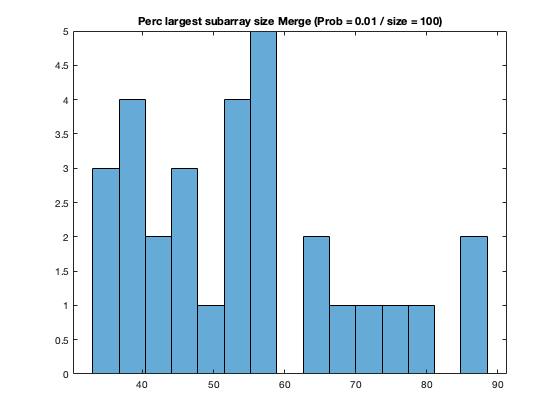
\includegraphics[scale=0.45]{figures/histogram_merge_LSS_001_100.png}}
     \textsf{\caption[Histogram for Mergesort.]{Histogram for Mergesort.\label{fig-histogram-mergesort-lss-001-100}}}
     \end{subfigure}%
     \begin{subfigure}{.5\textwidth}
     \centering
     \frame{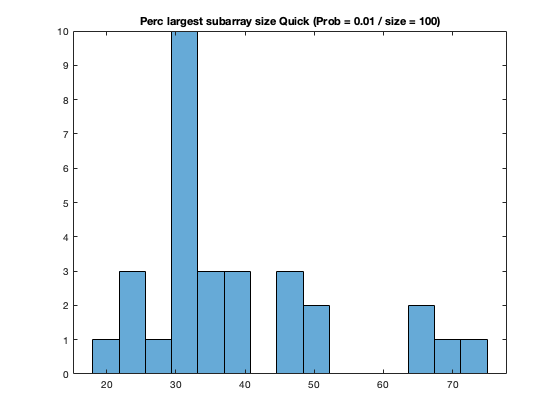
\includegraphics[scale=0.45]{figures/histogram_quick_LSS_001_100.png}}
     \textsf{\caption[Histogram for Quicksort.]{Histogram for Quicksort.\label{fig-histogram-quicksort-lss-001-100}}}
     \end{subfigure}
     \caption{Histograms for \%LSS, with \textit{probability of failure} of 0.01 and \textit{array size} of 100.}
    \label{fig-histogram-lss-001-100}
  \end{figure}

Based on Figures \ref{fig-histogram-lss-001-100}, \ref{fig-histogram-ueq-001-100} and \ref{fig-boxplots-001-100}, the following Tables \ref{tab-distribution-depentent-variable-ueq} and \ref{tab-distribution-depentent-variable-lss} illustrates the information about the dependent variables (\%LSS and \%UEQ) distribution.

\begin{table}[H]
    \caption{Dependent variable \%UEQ distribution.}
    \begin{center}
    \begin{tabular}{|c|c|c|c|c|c|c|c|}
    \hline
    \textbf{Prob. of Failure} & \textbf{Array Size} & \textbf{Algorithm} & \multicolumn{5}{|c|}{\textbf{Percentage of unordered elements quantity (\%UEQ)}} \\
    \cline{4-8} 
    & & & \textbf{\textit{Mean}}& \textbf{\textit{Median}} & \textbf{\textit{Std. Deviation}} & \textbf{\textit{Minimum}} & \textbf{\textit{Maximum}} \\
    \hline
    0.01 & 100 & bubble & 3.07 & 3.0 & 1.64 & 0.0 & 6.0 \\
    \hline
    0.01 & 100 & insertion & 10.87 & 11.0 & 1.59 & 8.0 & 14.0 \\
    \hline
    0.05 & 10000 & merge & 28.32 & 28.34 & 0.31 & 27.69 & 28.86 \\
    \hline
    0.05 & 10000 & quick & 19.56 & 19.58 & 0.26 & 18.95 & 20.07 \\
    \hline
    \end{tabular}
    \label{tab-distribution-depentent-variable-ueq}
    \end{center}
\end{table}

\begin{figure}[H]
    \centering
     \begin{subfigure}{.5\textwidth}
     \centering
     \frame{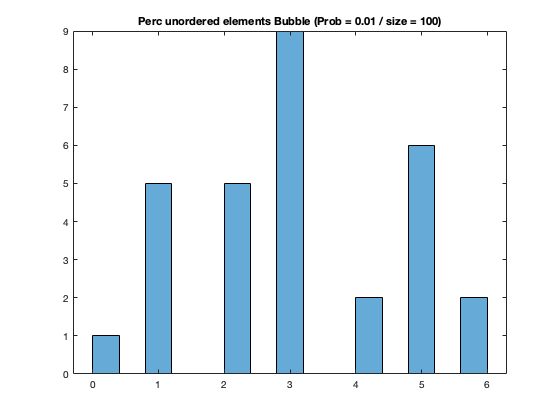
\includegraphics[scale=0.45]{figures/histogram_bubble_UEQ_001_100.png}}
     \textsf{\caption[Histogram for Bubblesort.]{Histogram for Bubblesort.\label{fig-histogram-bubble-ueq-001-100}}}
     \end{subfigure}%
     \begin{subfigure}{.5\textwidth}
     \centering
     \frame{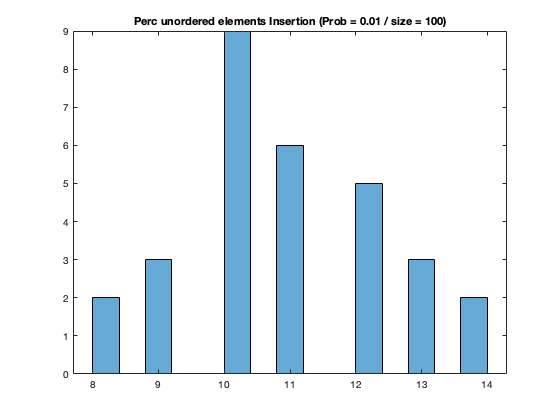
\includegraphics[scale=0.45]{figures/histogram_insertion_UEQ_001_100.png}}
     \textsf{\caption[Histogram for Bubblesort.]{Histogram for Bubblesort.\label{fig-histogram-insertion-ueq-001-100}}}
     \end{subfigure}
     \begin{subfigure}{.5\textwidth}
     \centering
     \frame{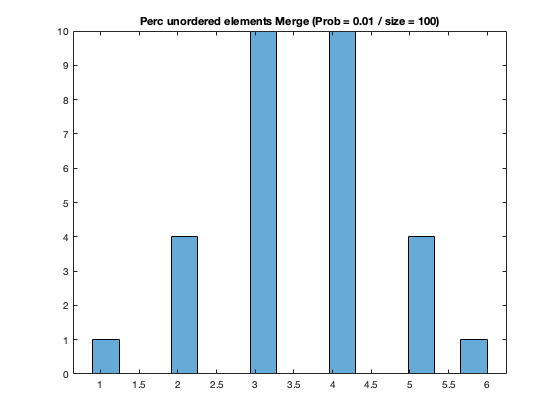
\includegraphics[scale=0.45]{figures/histogram_merge_UEQ_001_100.png}}
     \textsf{\caption[Histogram for Mergesort.]{Histogram for Mergesort.\label{fig-histogram-mergesort-ueq-001-100}}}
     \end{subfigure}%
     \begin{subfigure}{.5\textwidth}
     \centering
     \frame{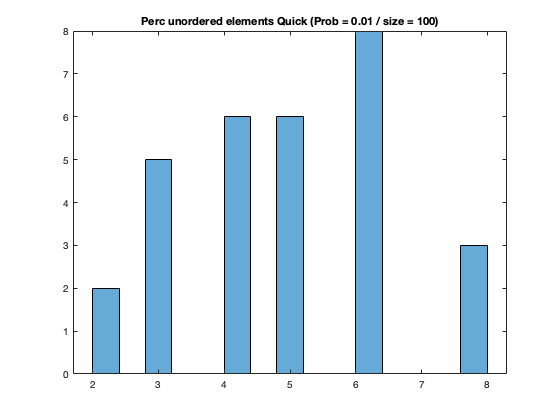
\includegraphics[scale=0.45]{figures/histogram_quick_UEQ_001_100.png}}
     \textsf{\caption[Histogram for Quicksort.]{Histogram for Quicksort.\label{fig-histogram-quicksort-ueq-001-100}}}
     \end{subfigure}
     \caption{Histograms for \%UEQ, with \textit{probability of failure} of 0.01 and \textit{array size} of 100.}
    \label{fig-histogram-ueq-001-100}
  \end{figure}

\begin{table}[H]
    \caption{Dependent variable \%LSS distribution.}
    \begin{center}
    \begin{tabular}{|c|c|c|c|c|c|c|c|}
    \hline
    \textbf{Prob. of Failure} & \textbf{Array Size} & \textbf{Algorithm} & \multicolumn{5}{|c|}{\textbf{Percentage of largest subarray size (\%LSS)}} \\
    \cline{4-8} 
    & & & \textbf{\textit{Mean}}& \textbf{\textit{Median}} & \textbf{\textit{Std. Deviation}} & \textbf{\textit{Minimum}} & \textbf{\textit{Maximum}} \\
    \hline
    0.01 & 100 & bubble & 67.4 & 71.0 & 15.84 & 38.0 & 100.0 \\
    \hline
    0.01 & 100 & insertion & 19.77 & 20.0 & 3.11 & 14.0 & 27.0 \\
    \hline
    0.05 & 10000 & merge & 0.19 & 0.2 & 0.03 & 0.15 & 28.86 \\
    \hline
    0.05 & 10000 & quick & 0.3 & 0.3 & 0.03 & 0.23 & 0.34 \\
    \hline
    \end{tabular}
    \label{tab-distribution-depentent-variable-lss}
    \end{center}
\end{table}

We produced graphs with the same data showed in Tables \ref{tab-distribution-depentent-variable-ueq} and \ref{tab-distribution-depentent-variable-lss}. Figure \ref{fig-distribution-all-algorithms-001-all-sizes} shows an example of these graphs. On it, we illustrate on the top-left graph that, considering the mean, bubblesort produces fewer unordered elements related to the total than other algorithms.

\begin{figure}[H]
    \centering
     \begin{subfigure}{.5\textwidth}
     \centering
     \frame{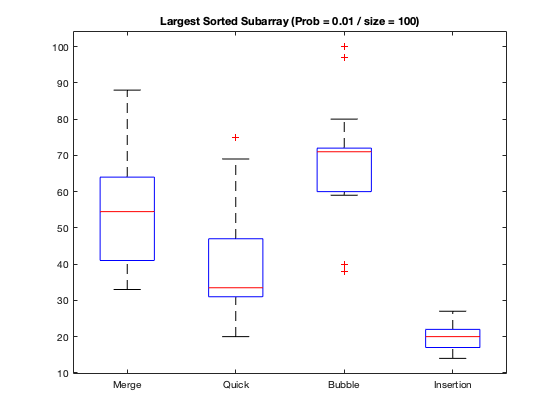
\includegraphics[scale=0.45]{figures/boxplot_lss_001_100.png}}
     \textsf{\caption[Boxplot for \%LSS.]{Boxplot for \%LSS.\label{fig-boxplot-lss-001-100}}}
     \end{subfigure}%
     \begin{subfigure}{.5\textwidth}
     \centering
     \frame{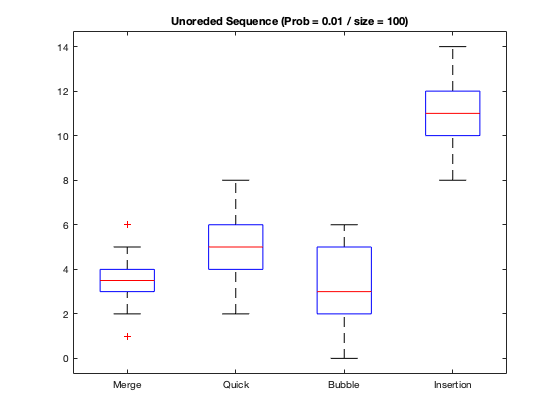
\includegraphics[scale=0.45]{figures/boxplot_ueq_001_100.png}}
     \textsf{\caption[Boxplot for \%UEQ.]{Boxplot for \%UEQ.\label{fig-boxplot-ueq-001-100}}}
     \end{subfigure}
     \caption{Boxplots for \%LSS and \%UEQ variables, with \textit{probability of failure} of 0.01 and \textit{array size} of 100.}
    \label{fig-boxplots-001-100}
\end{figure}

\begin{figure}[H]
    \centering
    \frame{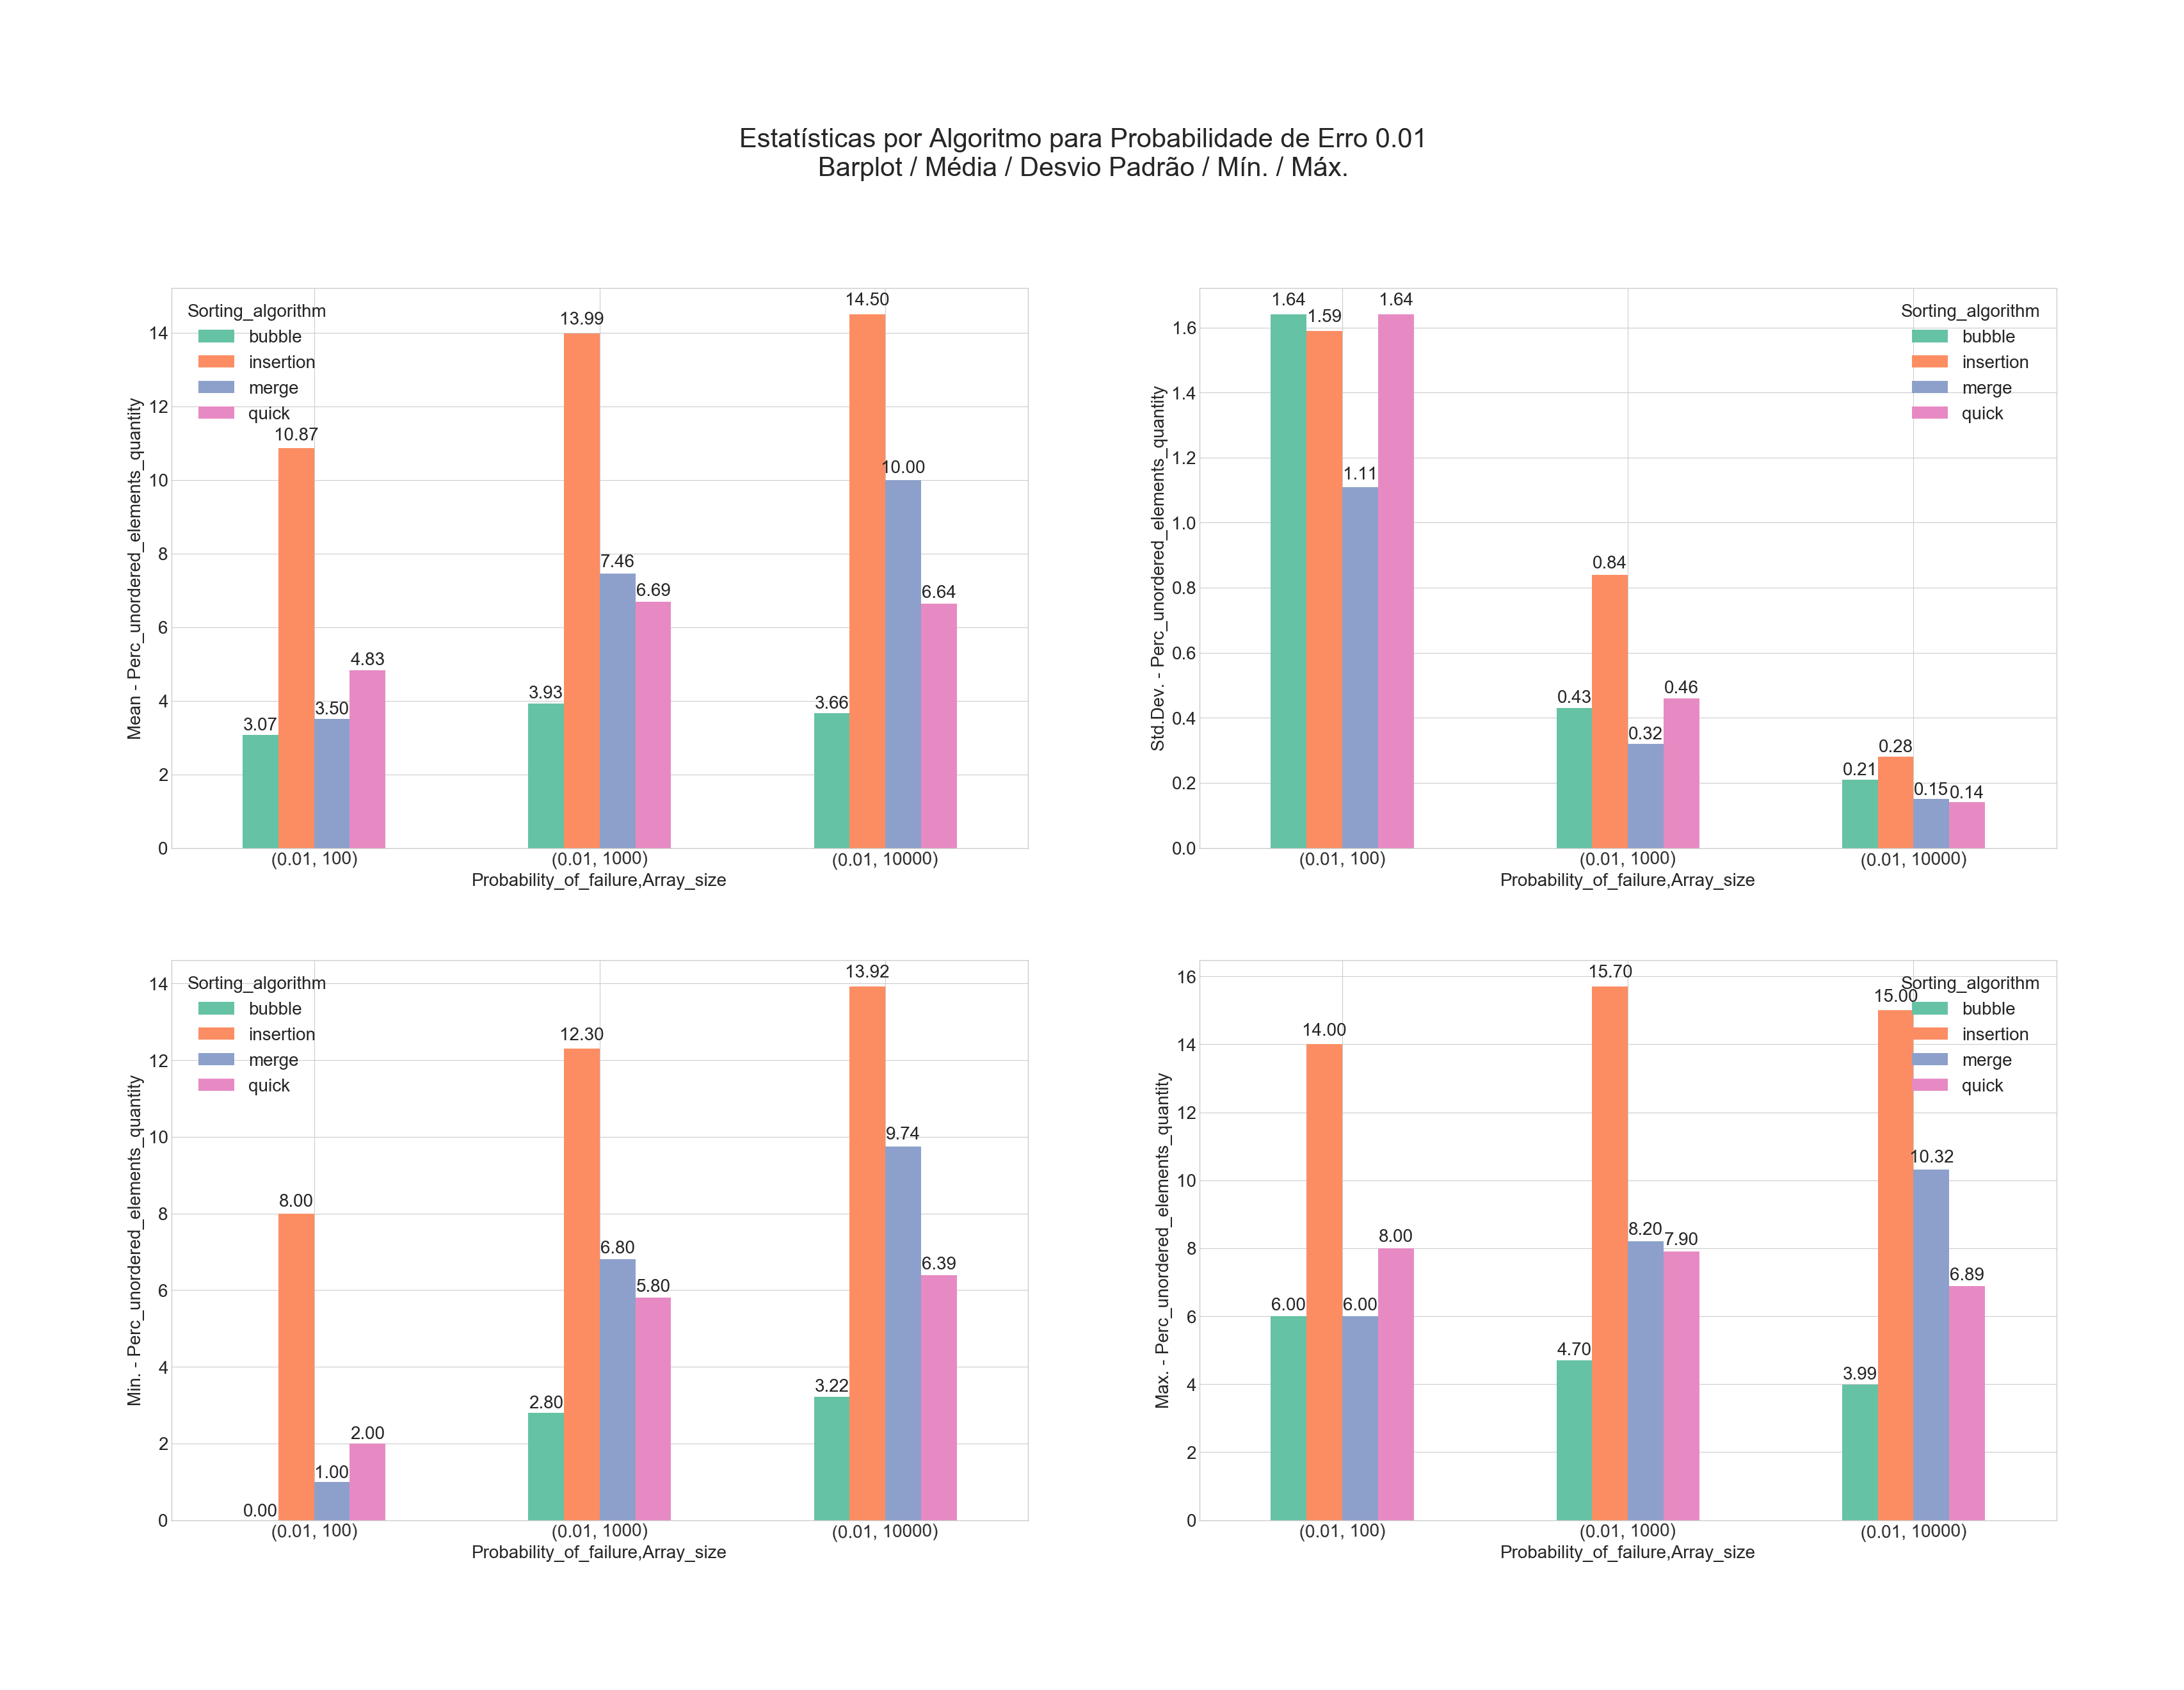
\includegraphics[scale=0.20]{figures/Estatisticas_por_Algoritmo_Prob_001.png}}
    \caption{Distribution data with \textit{probability of failure} of 0.01, all algorithms and \textit{array sizes}.}
    \label{fig-distribution-all-algorithms-001-all-sizes}
\end{figure}

\subsection{Dependent Variables Normality}

An essential step to continue the analysis is to verify if dependent variables have a normal distribution. In this work, we produced the Q-Q plot to analyze the normality visually. We also ran the Shapiro-Wilk \cite{shapiro1965analysis} test to confirm if they follow a normal distribution or not.

After the Shapiro-Wilk test, we determine that only the dependent variable \%UEQ (\textit{percentage of unordered elements quantity}) has a normal distribution related to mean for all algorithms. This situation occurred considering all possible combinations between independent variables: \textit{sorting algorithm}, \textit{probability of failure} and \textit{array size}.

Based on these results, we choose to test just the hypothesis associated with the dependent variable \%UEQ. We made use of the ANOVA method to test the hypothesis, and this method is premised the normal distribution of variables values.

Tables \ref{table-shapiro-test-lss-001-100} and \ref{table-shapiro-test-ueq-001-100} shows examples of results we got running Shapiro-Wilk test. The independent variables assume these values: \textit{probability of failure} of 0.01 and \textit{array size} of 100. The bold \textit{p-values} confirms that the data is normally distributed.

\begin{table}[H]
    \parbox{.45\linewidth}{
        \caption{Shapiro-Wilk test for \%LSS with \textit{probability of failure} of 1\% and \textit{array size} of 100.}
        \begin{center}
        \begin{tabular}{|c|c|c|}
        \hline
        \textbf{Algorithm} & \textbf{W} & \textbf{p-value} \\
        \hline
        Bubblesort & 0.854840 & 0.0007 \\
        \hline
        Insertion Sort & 0.961790 & \textbf{0.3439} \\
        \hline
        Mergesort & 0.937173 & \textbf{0.0763} \\
        \hline
        Quicksort & 0.869708 & 0.0016 \\
        \hline
        \end{tabular}
        \label{table-shapiro-test-lss-001-100}
        \end{center}
    }
    \hfill
    \parbox{.45\linewidth}{
        \caption{Shapiro-Wilk test for \%UEQ with \textit{probability of failure} of 1\% and \textit{array size} of 100.}
        \begin{center}
        \begin{tabular}{|c|c|c|}
        \hline
        \textbf{Algorithm} & \textbf{W} & \textbf{p-value} \\
        \hline
        Bubblesort & 0.934980 & \textbf{0.0666} \\
        \hline
        Insertion Sort & 0.949881 & \textbf{0.1678} \\
        \hline
        Mergesort & 0.936667 & \textbf{0.0739} \\
        \hline
        Quicksort & 0.936049 & \textbf{0.0712} \\
        \hline
        \end{tabular}
        \label{table-shapiro-test-ueq-001-100}
        \end{center}
    }
\end{table}

Q-Q plot shows that how much more blue points close to the red line, most normal is the distribution. Figure \ref{fig-qqplot-lss-001-100} below presents this graph for the dependent variable \textit{percentage of the largest subarray size} considering a \textit{probability of failure} of 1\% and a \textit{array size} of 100 for all sorting algorithms. 

\begin{figure}[H]
    \centering
    \frame{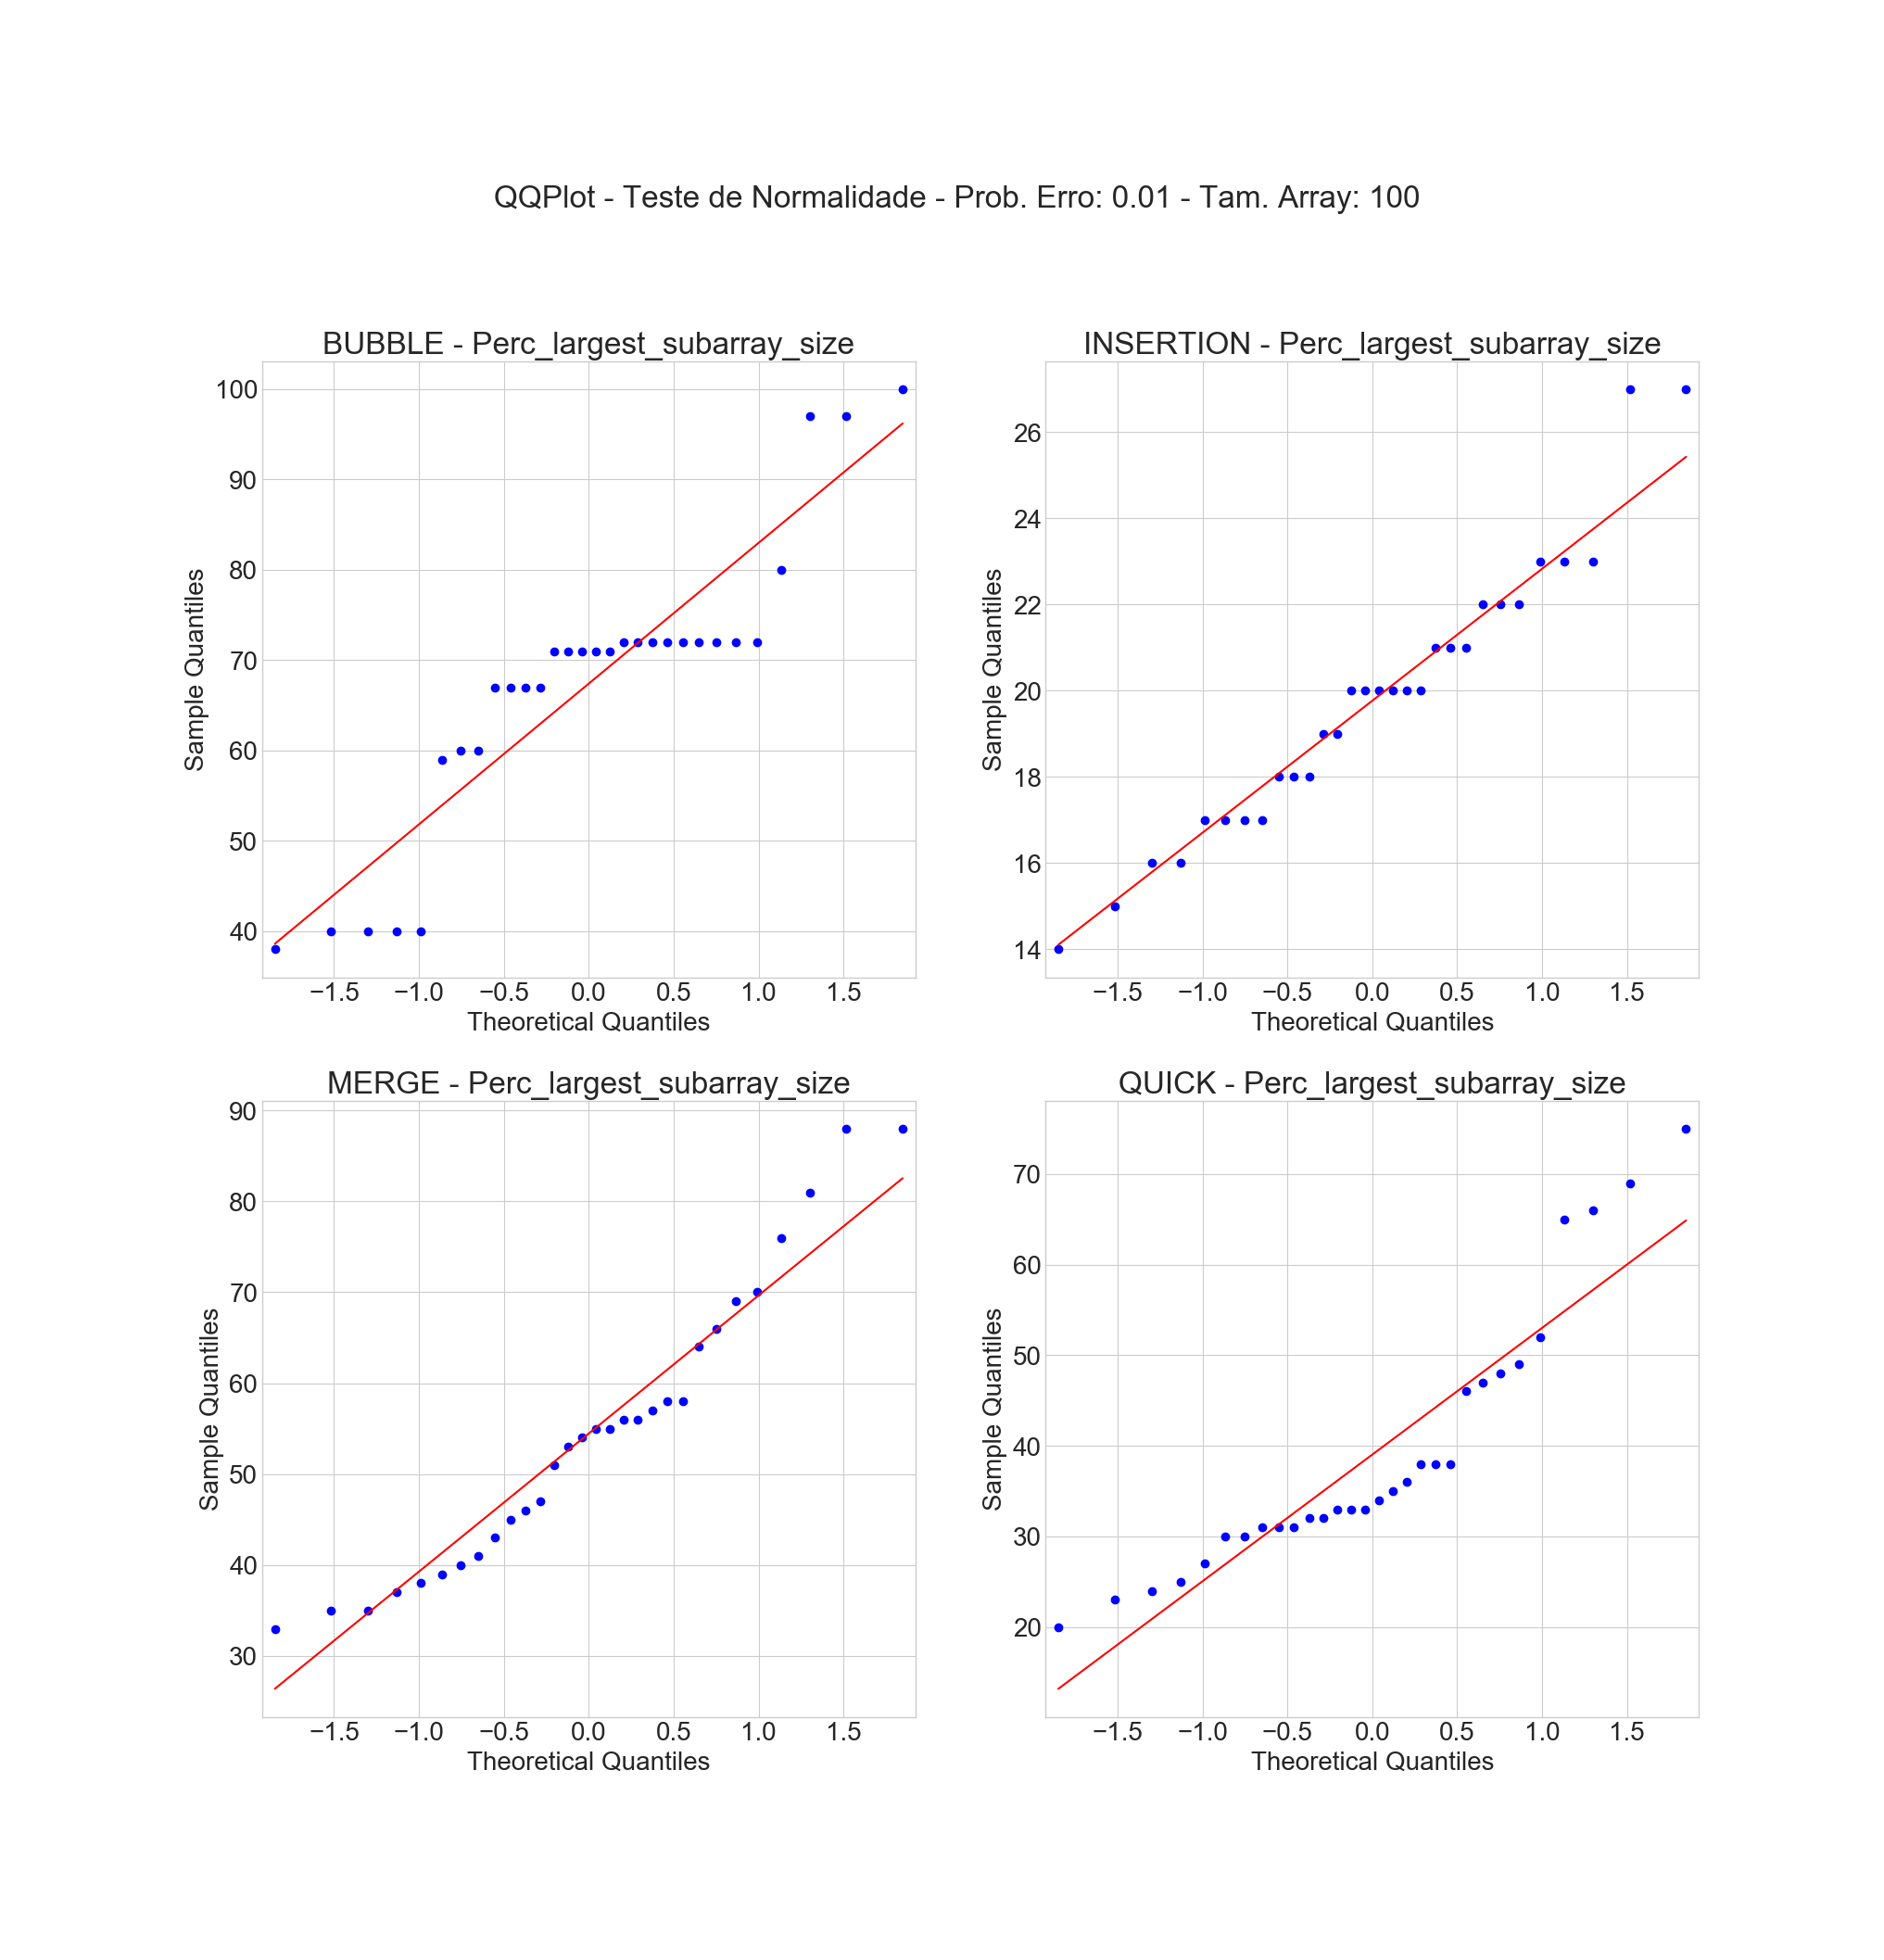
\includegraphics[scale=0.30]{figures/anova_prob_0_01_tam_100_Perc_largest_subarray_size.png}}
    \textsf{\caption[Q-Q plot for \%LSS with \textit{probability of failure} of 1\% and \textit{array size} of 100.]{Q-Q plot for \%LSS with \textit{probability of failure} of 1\% and \textit{array size} of 100.\label{fig-qqplot-lss-001-100}}}
 \end{figure}

 Figure \ref{fig-qqplot-ueq-001-100} shows the same graph for the dependent variable \textit{percentage of unordered elements quantity} considering same values for independent variables.

\begin{figure}[H]
    \centering
    \frame{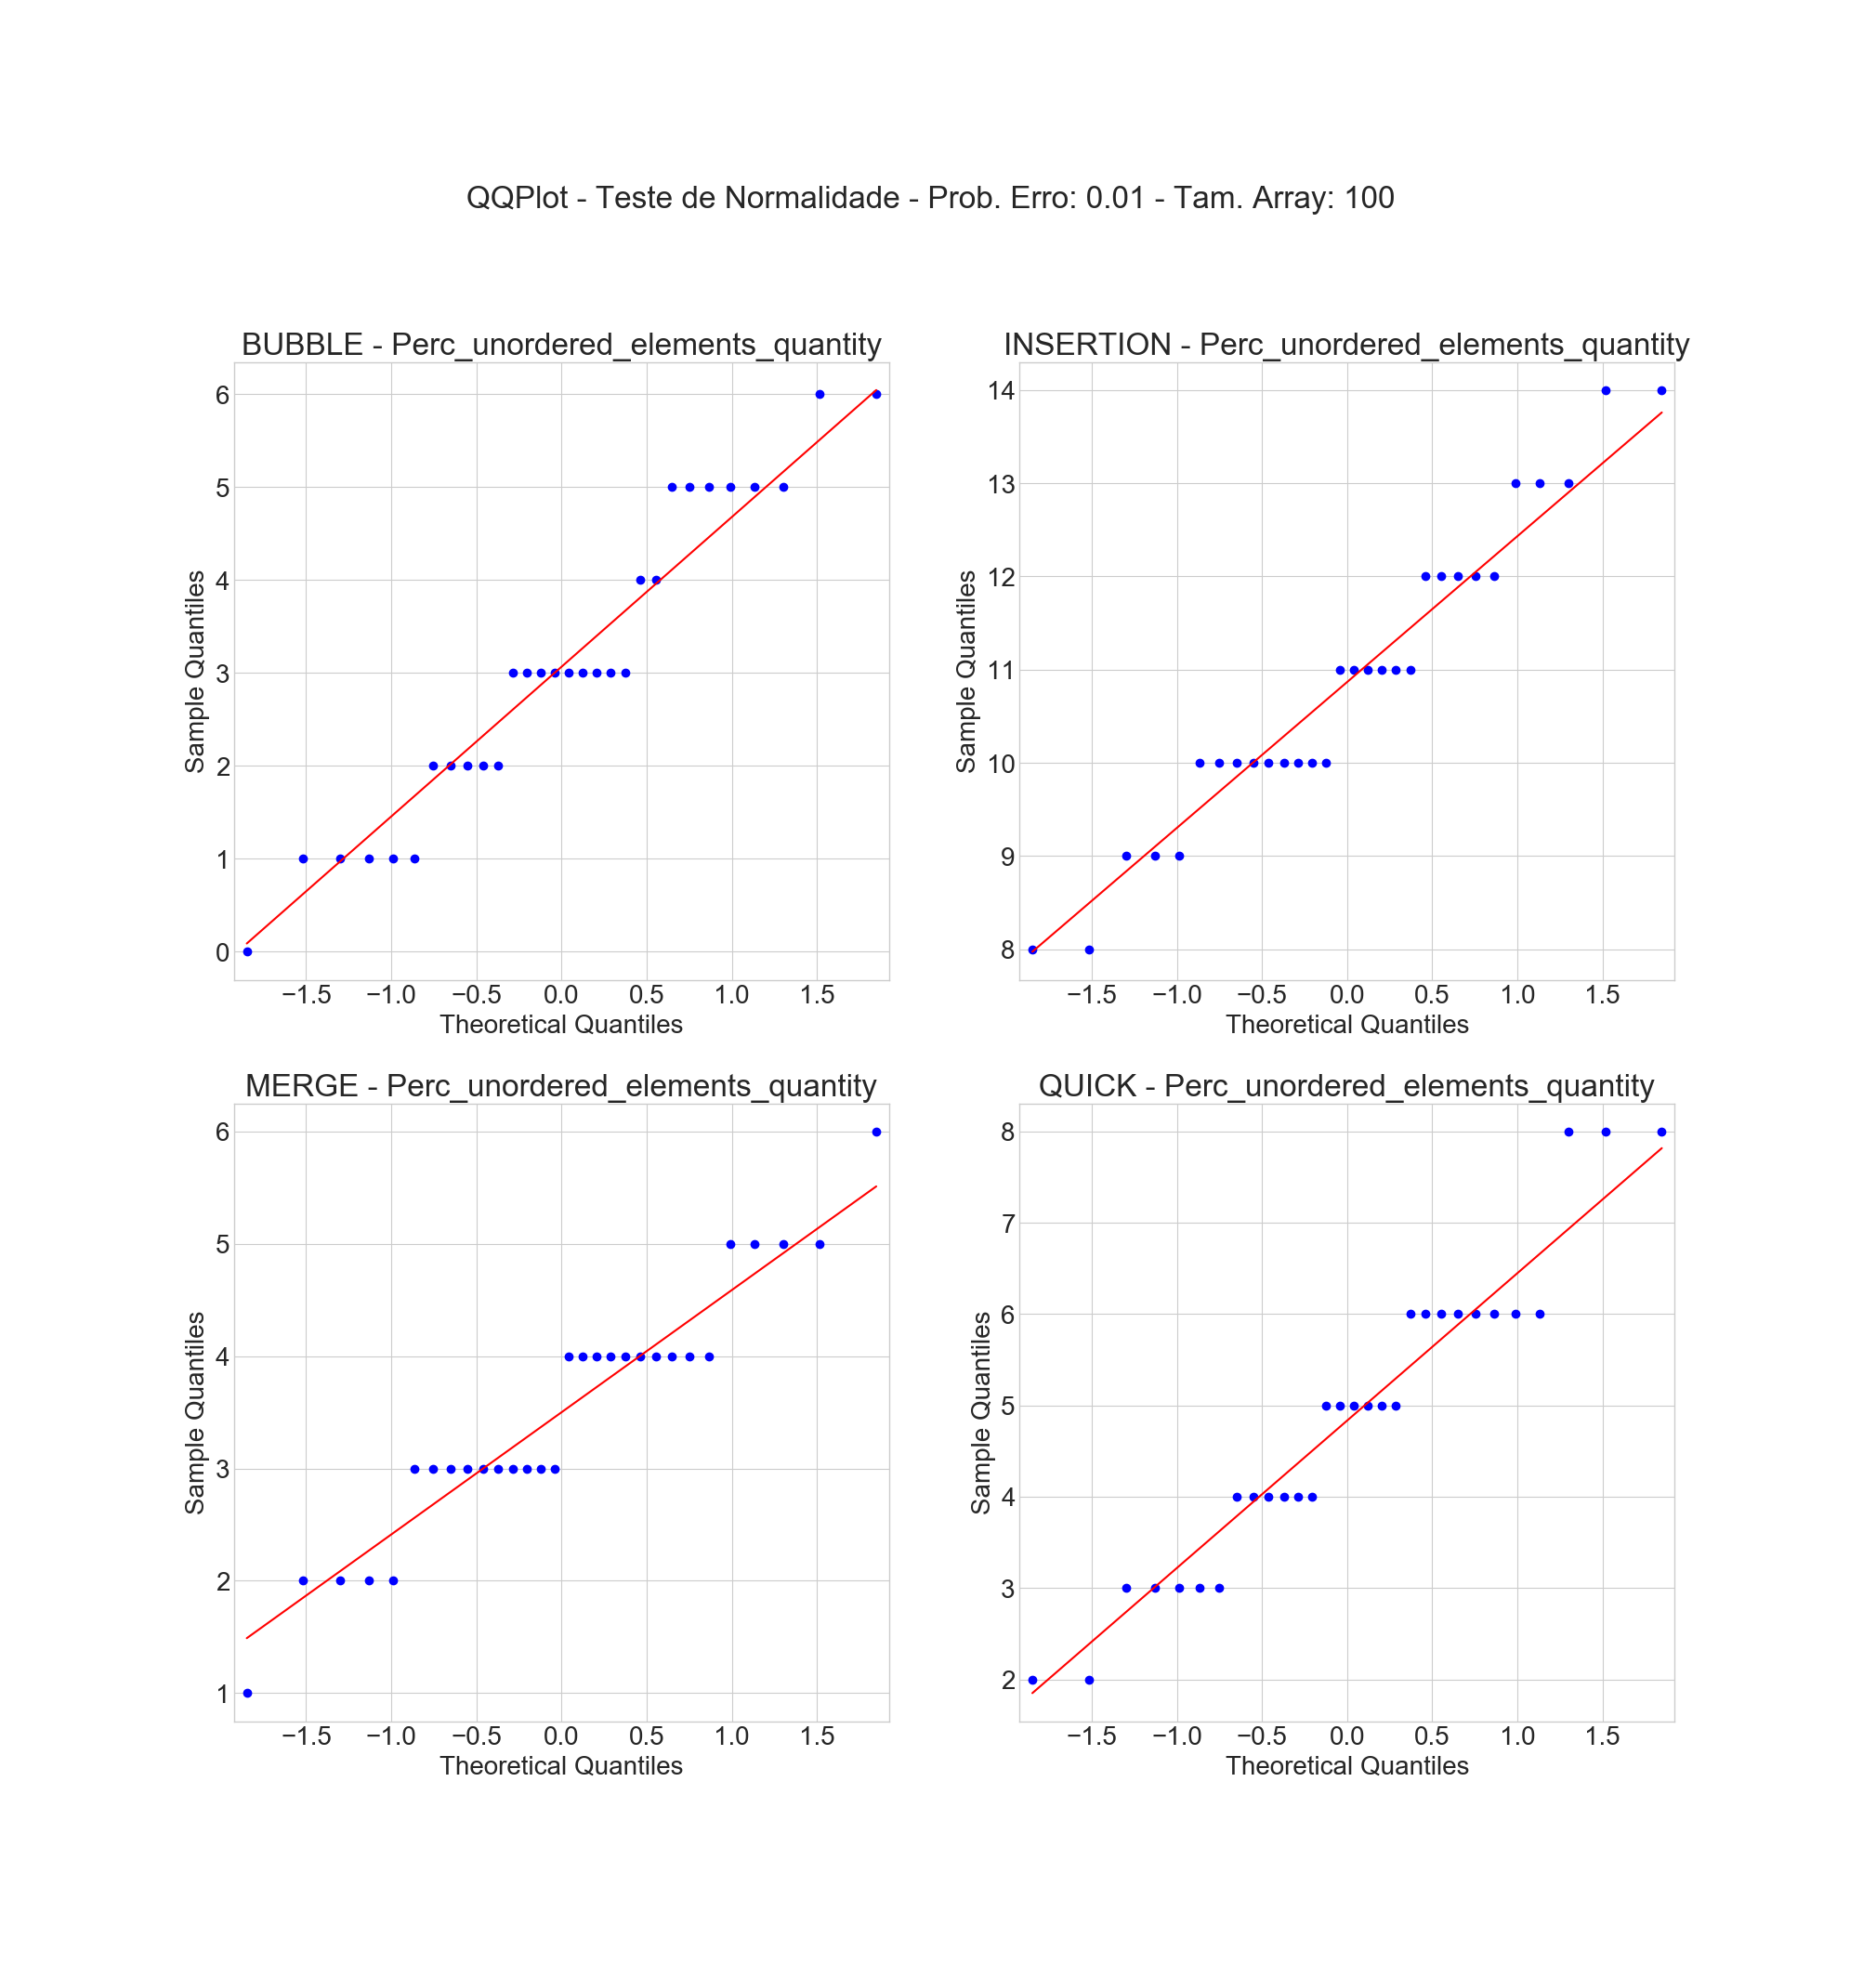
\includegraphics[scale=0.30]{figures/anova_prob_0_01_tam_100_Perc_unordered_elements_quantity.png}}
    \textsf{\caption[Q-Q plot for \%UEQ with \textit{probability of failure} of 1\% and \textit{array size} of 100.]{Q-Q plot for \%UEQ with \textit{probability of failure} of 1\% and \textit{array size} of 100.\label{fig-qqplot-ueq-001-100}}}
\end{figure}

Tables \ref{table-shapiro-test-lss-005-1000} and \ref{table-shapiro-test-ueq-005-1000} shows another examples of results we got running Shapiro-Wilk test. The independent variables assume these values: \textit{probability of failure} of 0.05 and \textit{array size} of 1000. The bold \textit{p-values} confirms that the data is normally distributed.

\begin{table}[H]
    \parbox{.45\linewidth}{
        \caption{Shapiro-Wilk test for \%LSS with \textit{probability of failure} of 5\% and \textit{array size} of 1000.}
        \begin{center}
        \begin{tabular}{|c|c|c|}
        \hline
        \textbf{Algorithm} & \textbf{W} & \textbf{p-value} \\
        \hline
        Bubblesort & 0.891642 & 0.0052 \\
        \hline
        Insertion Sort & 0.921918 & 0.0300 \\
        \hline
        Mergesort & 0.878308 & 0.0025 \\
        \hline
        Quicksort & 0.917583 & 0.0232 \\
        \hline
        \end{tabular}
        \label{table-shapiro-test-lss-005-1000}
        \end{center}
    }
    \hfill
    \parbox{.45\linewidth}{
        \caption{Shapiro-Wilk test for \%UEQ with \textit{probability of failure} of 5\% and \textit{array size} of 1000.}
        \begin{center}
        \begin{tabular}{|c|c|c|}
        \hline
        \textbf{Algorithm} & \textbf{W} & \textbf{p-value} \\
        \hline
        Bubblesort & 0.936459 & \textbf{0.0730} \\
        \hline
        Insertion Sort & 0.931681 & \textbf{0.0544} \\
        \hline
        Mergesort & 0.961920 & \textbf{0.3465} \\
        \hline
        Quicksort & 0.963954 & \textbf{0.3892} \\
        \hline
        \end{tabular}
        \label{table-shapiro-test-ueq-005-1000}
        \end{center}
    }
\end{table}

Other examples of distribution normality can be seen in Q-Q plot in Figures \ref{fig-qqplot-lss-005-1000} and Y below. The considered dependent variable is \textit{percentage of the largest subarray size} with a \textit{probability of failure} value of 5\% and \textit{array size} value of 10000 for all sorting algorithms.

\begin{figure}[H]
    \centering
    \frame{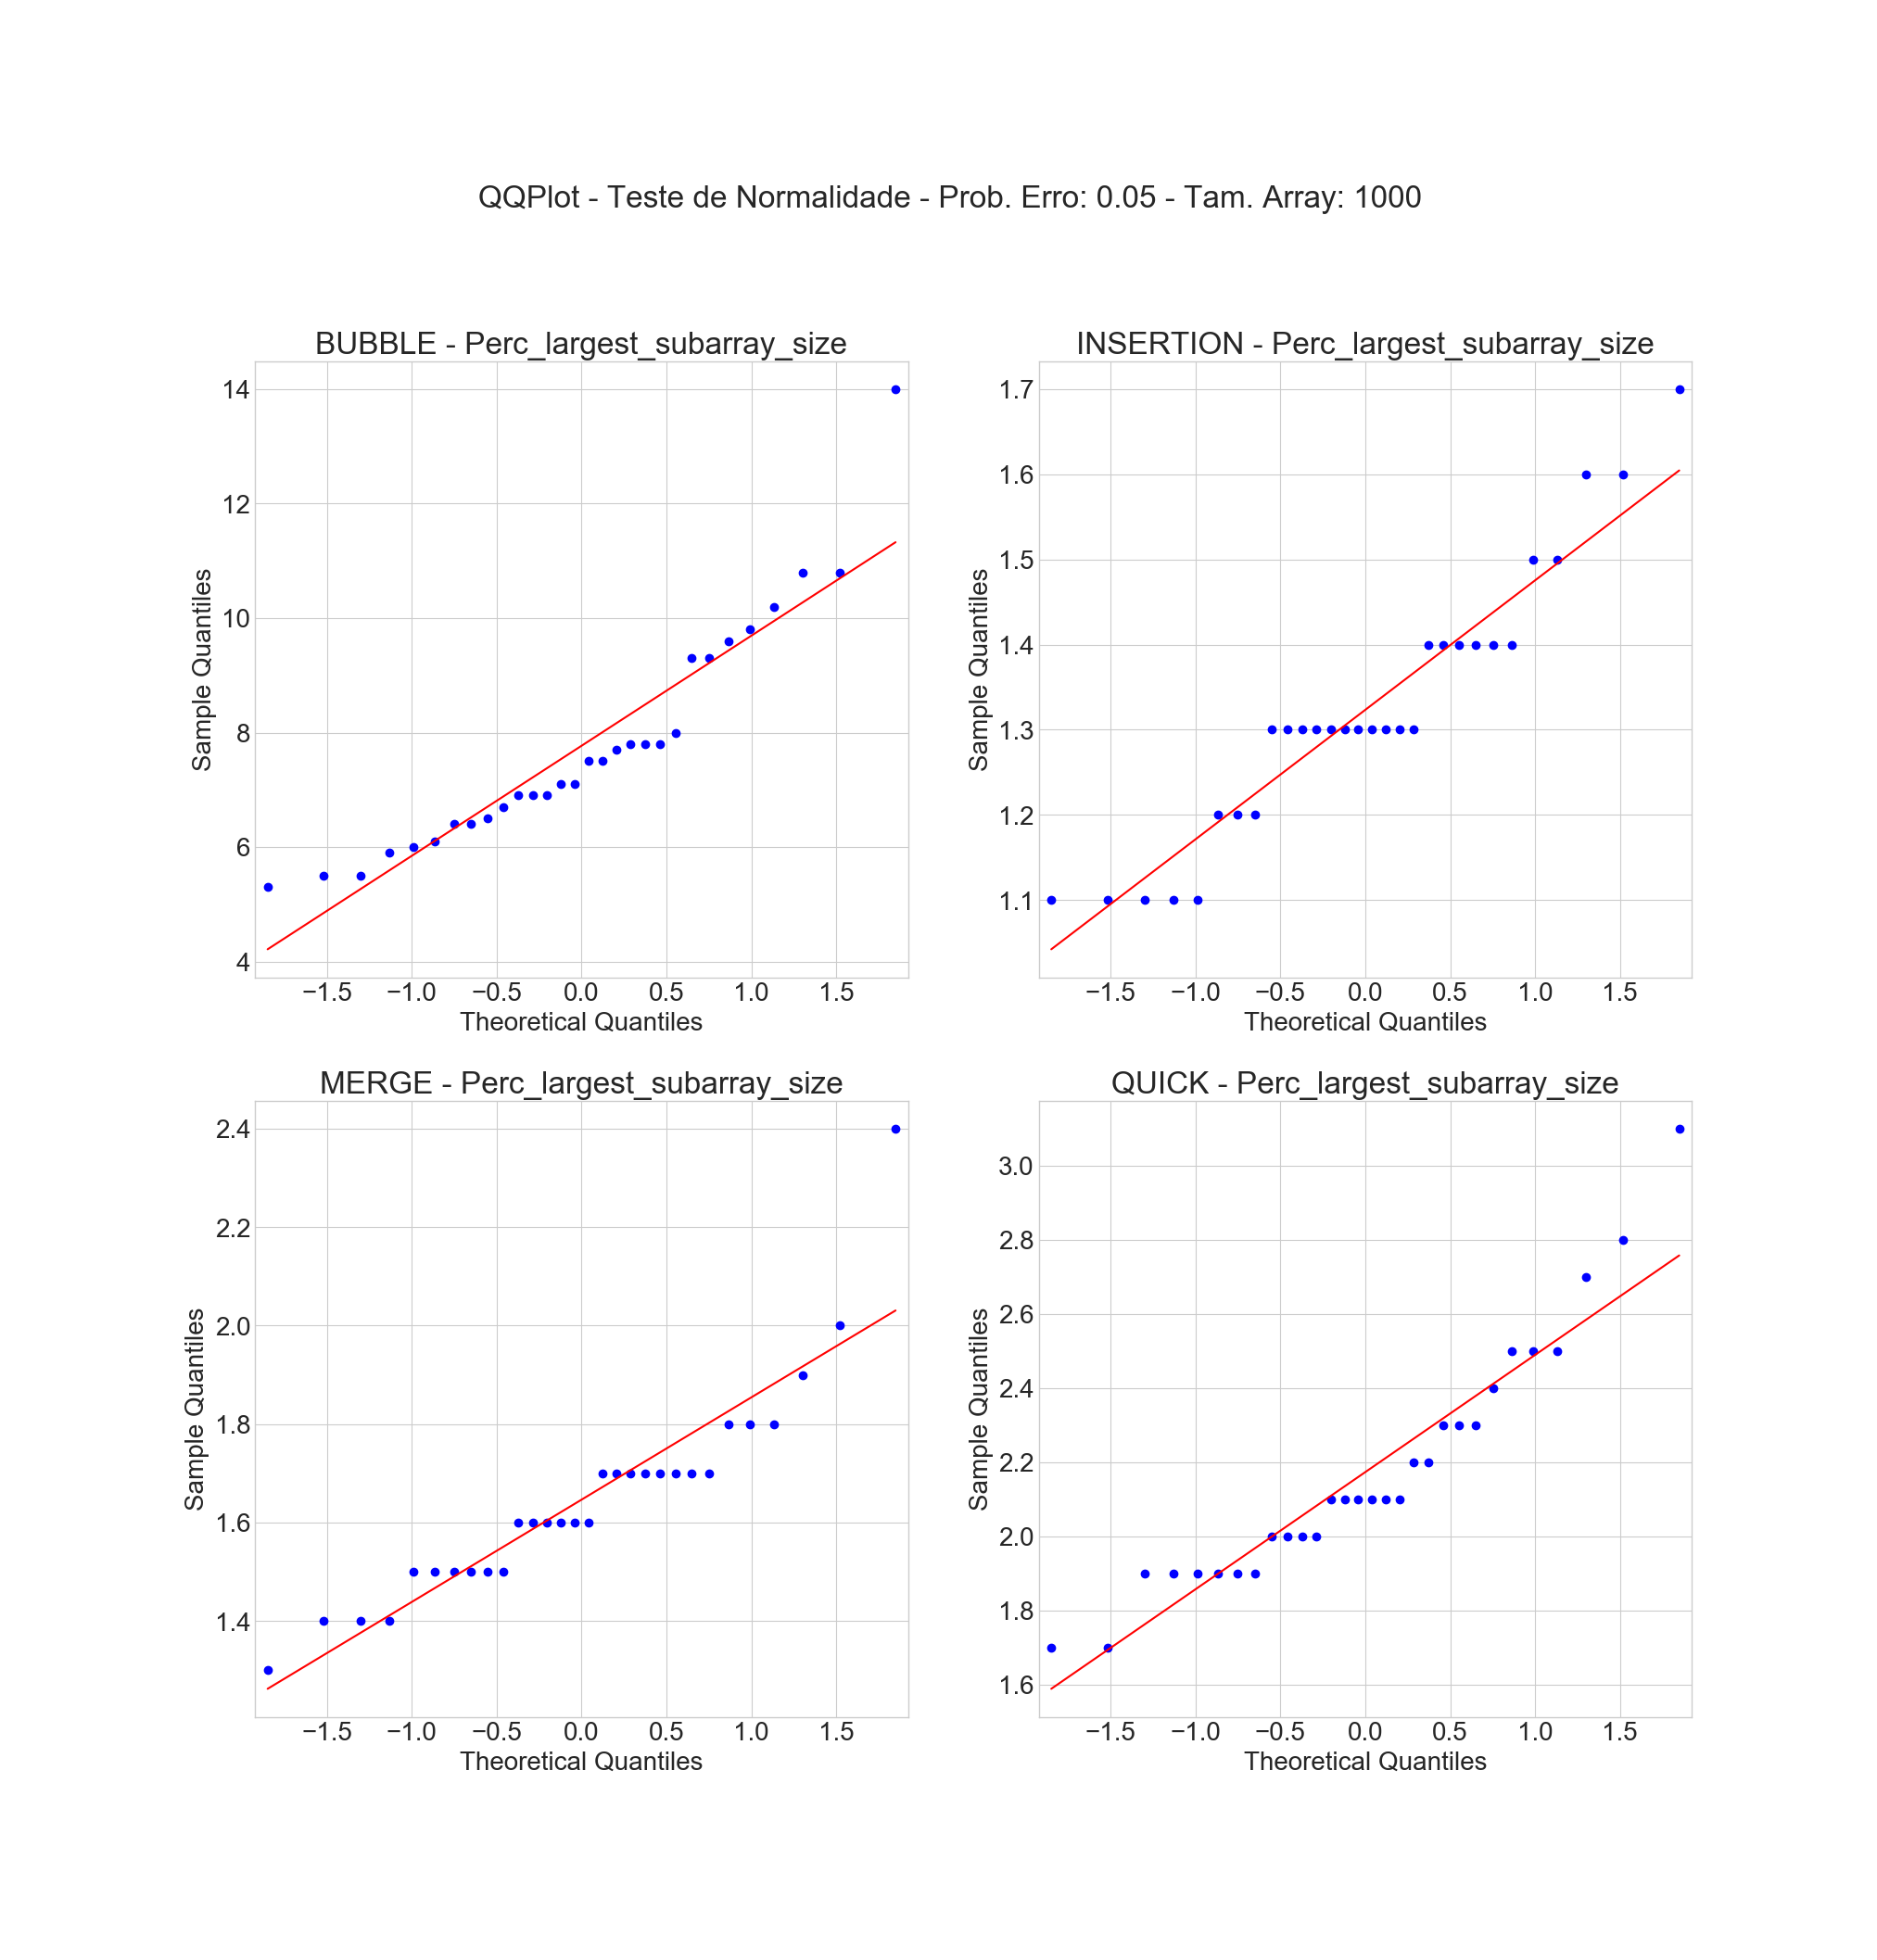
\includegraphics[scale=0.30]{figures/anova_prob_0_05_tam_1000_Perc_largest_subarray_size.png}}
    \textsf{\caption[Q-Q plot for \%LSS with \textit{probability of failure} of 5\% and \textit{array size} of 1000.]{Q-Q plot for \%LSS with \textit{probability of failure} of 5\% and \textit{array size} of 1000.\label{fig-qqplot-lss-005-1000}}}
 \end{figure}

 \begin{figure}[H]
    \centering
    \frame{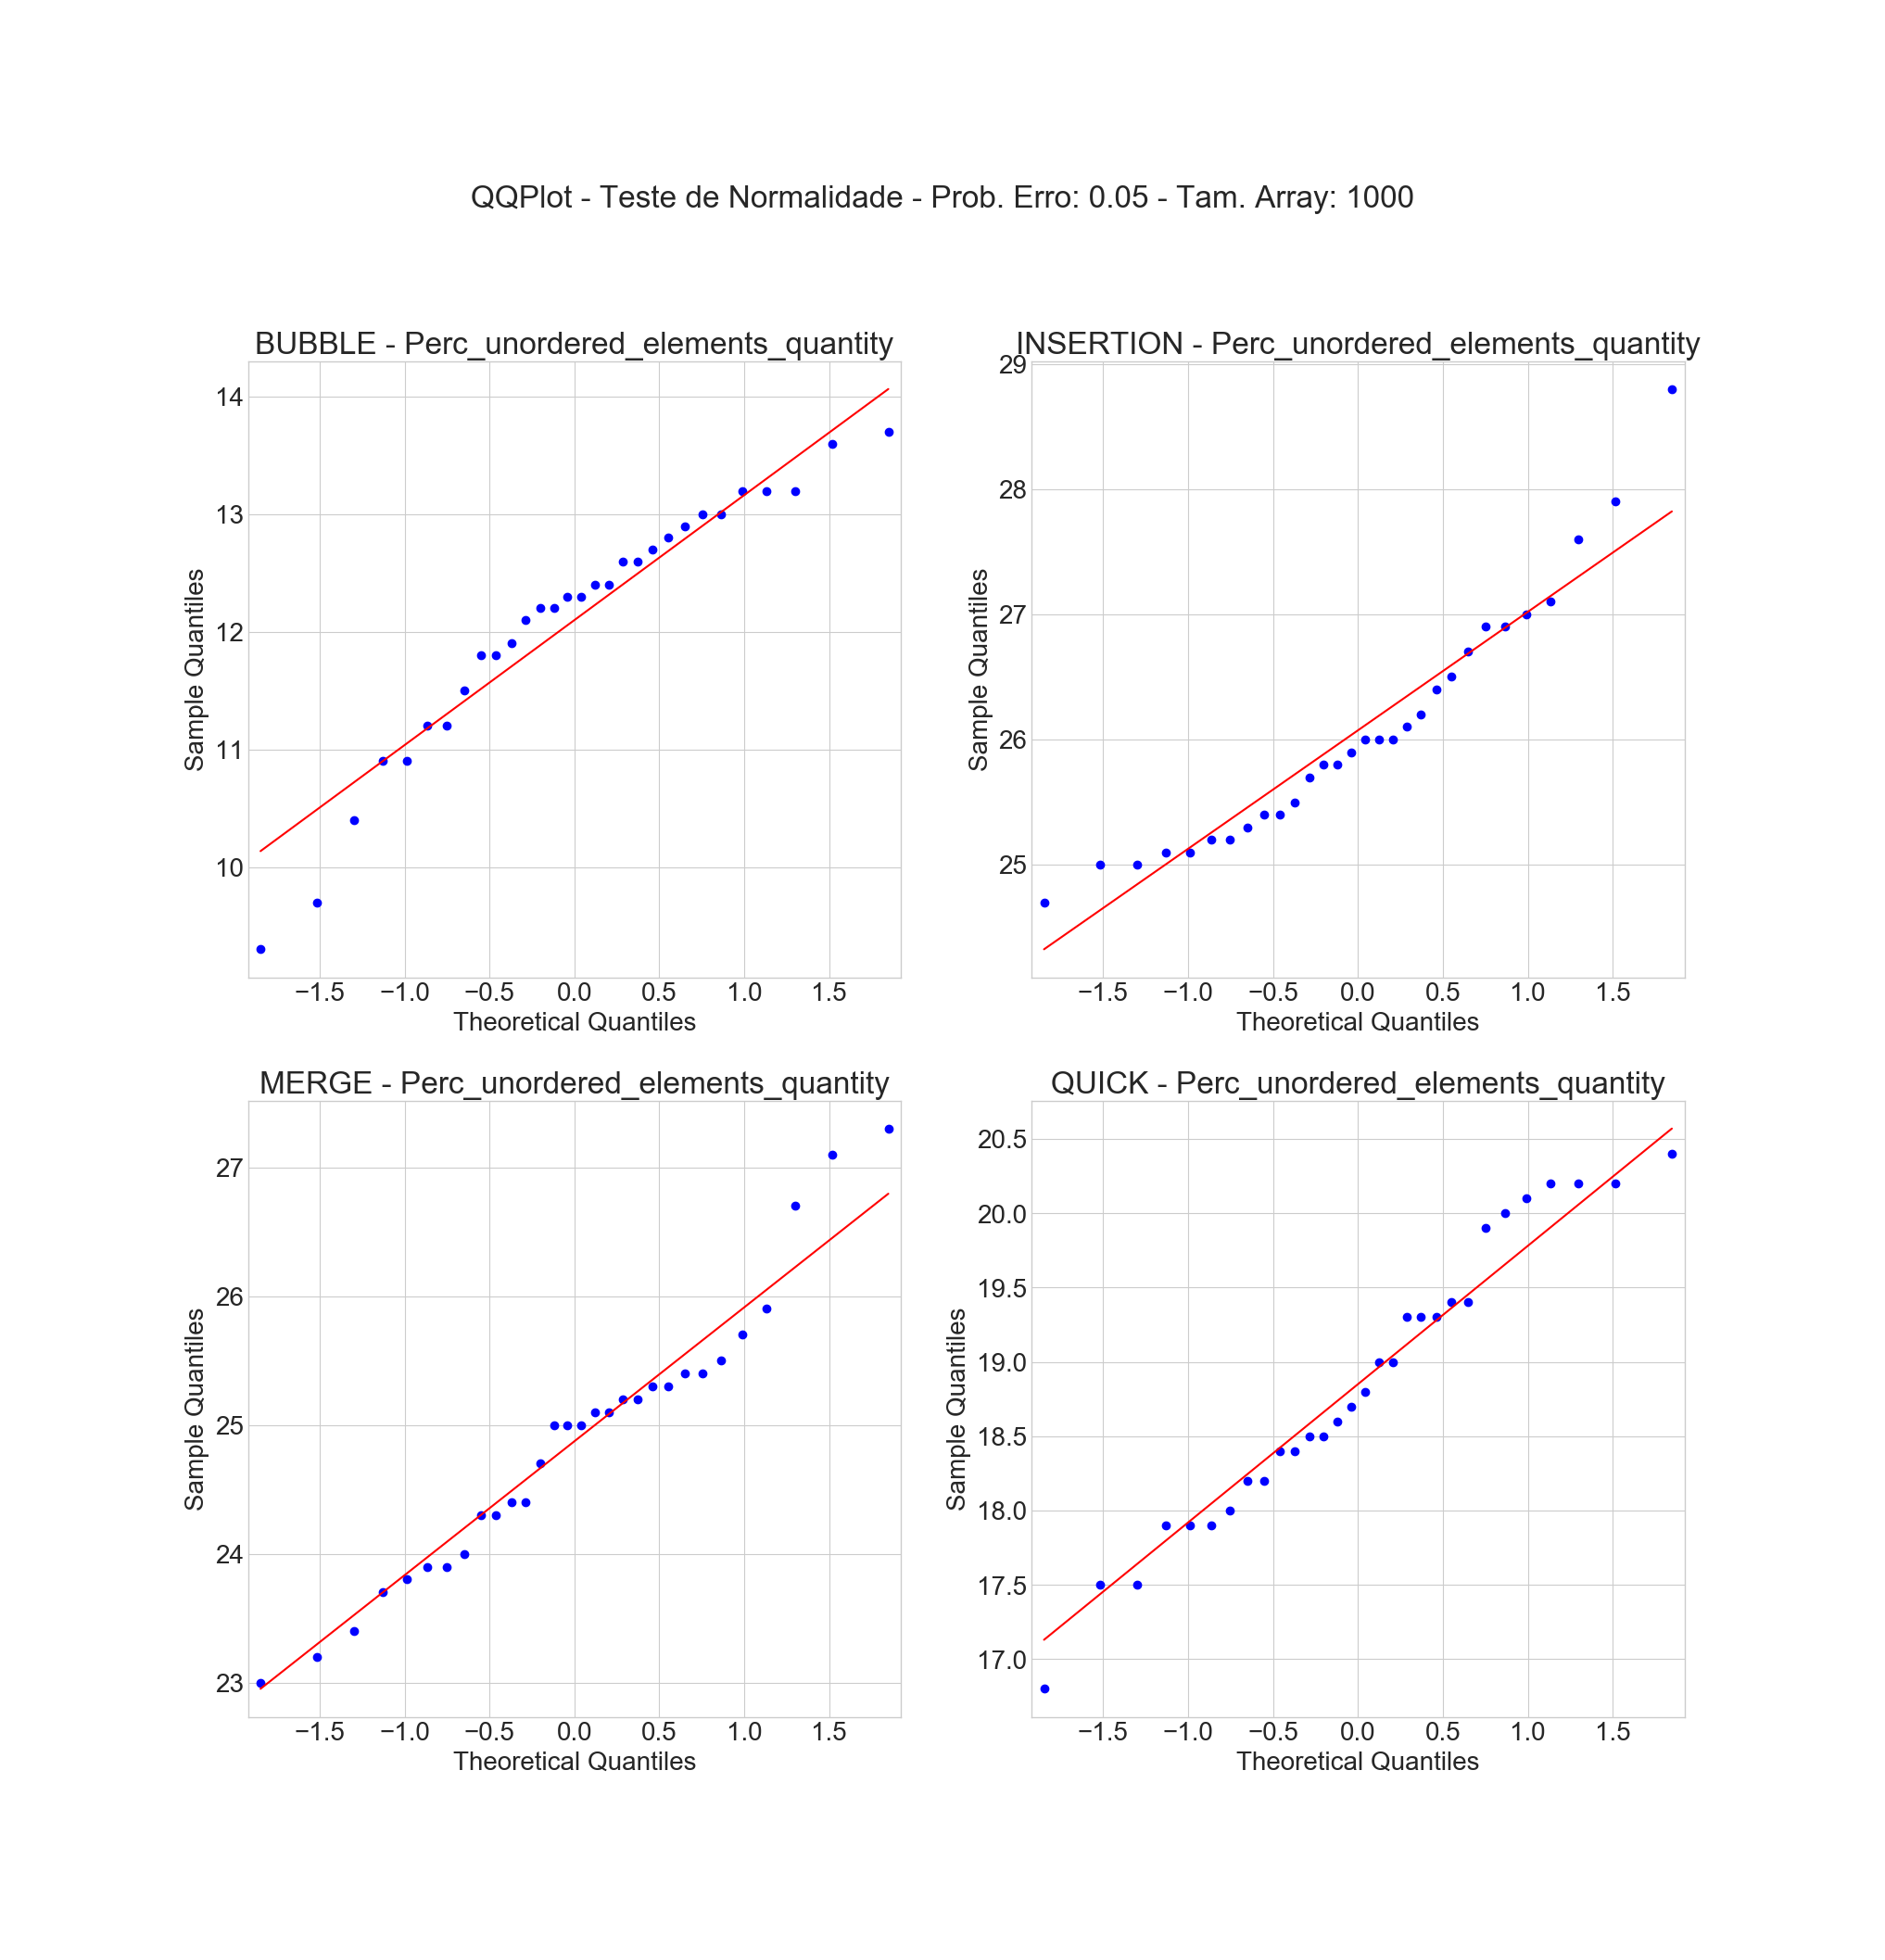
\includegraphics[scale=0.30]{figures/anova_prob_0_05_tam_1000_Perc_unordered_elements_quantity.png}}
    \textsf{\caption[Q-Q plot for \%UEQ with \textit{probability of failure} of 5\% and \textit{array size} of 1000.]{Q-Q plot for \%UEQ with \textit{probability of failure} of 5\% and \textit{array size} of 1000.\label{fig-qqplot-ueq-005-1000}}}
 \end{figure}

 \subsection{Hypothesis Testing}

 For hypothesis testing, we define a confidence degree of 95\%. As mentioned before, we only tested the hypothesis related to the dependent variable \%UEQ \textit{percentage of unordered elements quantity}. The hypothesis was:
 \begin{itemize}
     \item \textbf{Hypothesis 1}: For a given probability of failure and array size, tested algorithms will produce a different percentage of unordered elements quantity;
     \item \textbf{Hypothesis 3}: For each algorithm, the array size and probability of failure have a significative impact on the percentage of unordered elements quantity.
 \end{itemize}

 Because our dataset has 3 independent variables, we perform ANOVA method to simplify the hypothesis testing. This method allows comparing various groups of variables at the same time.

 \subsubsection{Testing Hypothesis 1}

We formulated the following hypothesis for the combination of independent variables \textit{probability of failure} and \textit{array size}:

\setcounter{hyp}{-1}
\begin{hyp} \label{hyp:a} There is no significant difference between algorithms related to variable \%UEQ.\end{hyp}
\begin{hyp} \label{hyp:b} There is significant difference between algorithms related to variable \%UEQ.\end{hyp}

After we run the testing method, we got the following results (Table \ref{tab-hypothesis1-testing}):

\begin{table}[H]
    \caption{Hypothesis 1 ANOVA results.}
    \begin{center}
    \begin{tabular}{|c|c|c|c|c|}
    \hline
    \multirow{2}{*}{\hfill}&\multicolumn{4}{|c|}{\textbf{Probablity of Failure = 1\% and Array Size = 100}} \\
    \cline{2-5}
    &\textbf{\textit{sum\_sq}} & \textbf{\textit{df}} & \textbf{\textit{F}} & \textbf{\textit{PR(>F)}} \\
    \hline
    algorithm & 1174.466667 & 3.0 & 171.368721 & \textbf{1.845762e-42} \\
    \hline
    residual & 265.000000 & 116.0 & & \\
    \hline
    \multirow{2}{*}{\hfill}&\multicolumn{4}{|c|}{\textbf{Probablity of Failure = 1\% and Array Size = 1000}} \\
    \cline{2-5}
    &\textbf{\textit{sum\_sq}} & \textbf{\textit{df}} & \textbf{\textit{F}} & \textbf{\textit{PR(>F)}} \\
    \hline
    algorithm & 1635.180250 & 3.0 & 1817.615579 & \textbf{2.610034e-97} \\
    \hline
    residual & 34.785667 & 116.0 & & \\
    \hline
    \multirow{2}{*}{\hfill}&\multicolumn{4}{|c|}{\textbf{Probablity of Failure = 1\% and Array Size = 10000}} \\
    \cline{2-5}
    &\textbf{\textit{sum\_sq}} & \textbf{\textit{df}} & \textbf{\textit{F}} & \textbf{\textit{PR(>F)}} \\
    \hline
    algorithm & 1948.204989 & 3.0 & 15831.708335 & \textbf{2.332995e-151} \\
    \hline
    residual & 4.758210 & 116.0 & & \\
    \hline
    \multirow{2}{*}{\hfill}&\multicolumn{4}{|c|}{\textbf{Probablity of Failure = 2\% and Array Size = 100}} \\
    \cline{2-5}
    &\textbf{\textit{sum\_sq}} & \textbf{\textit{df}} & \textbf{\textit{F}} & \textbf{\textit{PR(>F)}} \\
    \hline
    algorithm & 1106.5 & 3.0 & 88.617785 & \textbf{7.054900e-30} \\
    \hline
    residual & 482.8 & 116.0 & & \\
    \hline
    \multirow{2}{*}{\hfill}&\multicolumn{4}{|c|}{\textbf{Probablity of Failure = 2\% and Array Size = 1000}} \\
    \cline{2-5}
    &\textbf{\textit{sum\_sq}} & \textbf{\textit{df}} & \textbf{\textit{F}} & \textbf{\textit{PR(>F)}} \\
    \hline
    algorithm & 2286.83025 & 3.0 & 1990.144336 & \textbf{1.507899e-99} \\
    \hline
    residual & 44.43100 & 116.0 & & \\
    \hline
    \multirow{2}{*}{\hfill}&\multicolumn{4}{|c|}{\textbf{Probablity of Failure = 2\% and Array Size = 10000}} \\
    \cline{2-5}
    &\textbf{\textit{sum\_sq}} & \textbf{\textit{df}} & \textbf{\textit{F}} & \textbf{\textit{PR(>F)}} \\
    \hline
    algorithm & 3081.306943 & 3.0 & 18442.105239 & \textbf{3.406264e-155} \\
    \hline
    residual & 6.460427 & 116.0 & & \\
    \hline
    \multirow{2}{*}{\hfill}&\multicolumn{4}{|c|}{\textbf{Probablity of Failure = 5\% and Array Size = 100}} \\
    \cline{2-5}
    &\textbf{\textit{sum\_sq}} & \textbf{\textit{df}} & \textbf{\textit{F}} & \textbf{\textit{PR(>F)}} \\
    \hline
    algorithm & 2274.291667 & 3.0 & 225.58173 & \textbf{3.104916e-48} \\
    \hline
    residual & 389.833333 & 116.0 & & \\
    \hline
    \multirow{2}{*}{\hfill}&\multicolumn{4}{|c|}{\textbf{Probablity of Failure = 5\% and Array Size = 1000}} \\
    \cline{2-5}
    &\textbf{\textit{sum\_sq}} & \textbf{\textit{df}} & \textbf{\textit{F}} & \textbf{\textit{PR(>F)}} \\
    \hline
    algorithm & 3704.037583 & 3.0 & 1202.21591 & \textbf{3.625400e-87} \\
    \hline
    residual & 119.132333 & 116.0 & & \\
    \hline
    \multirow{2}{*}{\hfill}&\multicolumn{4}{|c|}{\textbf{Probablity of Failure = 5\% and Array Size = 10000}} \\
    \cline{2-5}
    &\textbf{\textit{sum\_sq}} & \textbf{\textit{df}} & \textbf{\textit{F}} & \textbf{\textit{PR(>F)}} \\
    \hline
    algorithm & 4948.821397 & 3.0 & 19487.120298 & \textbf{1.402080e-156} \\
    \hline
    residual & 9.819533 & 116.0 & & \\
    \hline
    \end{tabular}
    \label{tab-hypothesis1-testing}
    \end{center}
\end{table}

Based on these results, we reject the null hypothesis ($H_{0}$) for all testing combinations. Therefore, we can affirm with 95\% of confidence that there is a significant difference between algorithms related do variable \%UEQ.

\subsubsection{Testing Hypothesis 3}

We formulated the following hypothesis for all algorithms considered in this work:

\setcounter{hyp}{-1}
\begin{hyp} \label{hyp:a} The values of variables \textit{probability of failure} and \textit{array size} don't have a significant impact on values of \%UEQ variable.\end{hyp}
\begin{hyp} \label{hyp:b} The values of variables \textit{probability of failure} and \textit{array size} have a significant impact on values of \%UEQ variable.\end{hyp}

After we run the testing method, we got the following results (Table \ref{tab-hypothesis3-testing}):

\begin{table}[H]
    \caption{Hypothesis 3 ANOVA results}
    \begin{center}
    \begin{tabular}{|c|c|c|c|c|}
    \hline
    \multirow{2}{*}{\hfill}&\multicolumn{4}{|c|}{\textbf{Bubblesort}} \\
    \cline{2-5}
    &\textbf{\textit{sum\_sq}} & \textbf{\textit{df}} & \textbf{\textit{F}} & \textbf{\textit{PR(>F)}} \\
    \hline
    size\_of\_array & 0.019548 & 2.0 & 0.01350 & \textbf{0.90759} \\
    \hline
    probability\_of\_failure & 3590.644437 & 2.0 & 2479.71637 & \textbf{7.570027e-137} \\
    \hline
    residual & 385.169623 & 266.0 & &  \\
    \hline
    \multirow{2}{*}{\hfill}&\multicolumn{4}{|c|}{\textbf{Mergesort}} \\
    \cline{2-5}
    &\textbf{\textit{sum\_sq}} & \textbf{\textit{df}} & \textbf{\textit{F}} & \textbf{\textit{PR(>F)}} \\
    \hline
    size\_of\_array & 1784.873256 & 2.0 & 383.585800 & \textbf{1.702008e-53} \\
    \hline
    probability\_of\_failure & 13009.963175 & 2.0 & 2795.961630 & \textbf{3.801570e-143} \\
    \hline
    residual & 1237.731651 & 266.0 & &  \\
    \hline
    \multirow{2}{*}{\hfill}&\multicolumn{4}{|c|}{\textbf{Quicksort}} \\
    \cline{2-5}
    &\textbf{\textit{sum\_sq}} & \textbf{\textit{df}} & \textbf{\textit{F}} & \textbf{\textit{PR(>F)}} \\
    \hline
    size\_of\_array & 121.551362 & 2.0 & 32.964196 & \textbf{2.556033e-08} \\
    \hline
    probability\_of\_failure & 5626.955128 & 2.0 & 1526.005558 & \textbf{3.457996e-112} \\
    \hline
    residual & 980.841817 & 266.0 & &  \\
    \hline
    \multirow{2}{*}{\hfill}&\multicolumn{4}{|c|}{\textbf{Insertionsort}} \\
    \cline{2-5}
    &\textbf{\textit{sum\_sq}} & \textbf{\textit{df}} & \textbf{\textit{F}} & \textbf{\textit{PR(>F)}} \\
    \hline
    size\_of\_array & 309.843991 & 2.0 & 75.905868 & \textbf{3.236586e-16} \\
    \hline
    probability\_of\_failure & 6806.075083 & 2.0 & 1667.358570 & \textbf{1.414758e-116} \\
    \hline
    residual & 1085.798822 & 116.0 & & \\
    \hline
    \end{tabular}
    \label{tab-hypothesis3-testing}
    \end{center}
\end{table}

Based on these results, we reject the null hypothesis ($H_{0}$) for algorithms Mergesort, Quicksort, and Insertion sort. Therefore, we can affirm with 95\% of confidence that the values of variables \textit{probability of failure} and \textit{array size} have a significant impact on values of \%UEQ variable.

For Bubblesort algorithm, however, there is no confidence to reject the null hypothesis ($H_{0}$). Analyzing the result, we can affirm with 95\% of confidence that the value of \textit{probability of failure} variable had a significant impact on the value of the dependent variable \%UEQ. But we can not affirm the same related to independent variable \textit{array size}. These results demonstrate that, for the Bubblesort algorithm, the array sizes used in this experiment were not decisive to define values concerning the percentage of unordered elements quantity.

\subsection{Performance analysis related to \textit{percentage of unordered elements quantity} variable}

In this section, we present an analysis of overall performance related to dependent variable \textit{percentage of unordered elements quantity}. To help this analysis, we show below 3 bar graphs, each of these for a different value of \textit{probability of failure} independent variable. These graphs show information about values of \%UEQ variable grouped by \textit{array size} and \textit{sorting algorithm} variables. Figures \ref{fig-barplot-pof-001}, \ref{fig-barplot-pof-002}, and \ref{fig-barplot-pof-005} below exhibit these graphs.

The bars in each graph represent the sample mean value for variable \%UEQ inside each group. Above each bar, there is a vertical line that indicates the lower and upper limits of a confidence interval for a significance level of 5\% ($\alpha = 0.05$).

\begin{figure}[H]
    \centering
    \frame{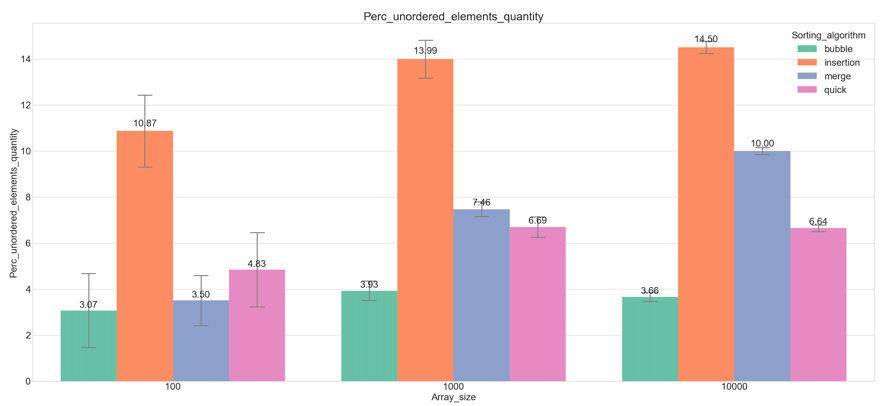
\includegraphics[scale=1.15]{figures/Barplot_Estatisticas_por_Algoritmo_Prob_0_01.png}}
    \textsf{\caption[Data for \textit{probability of failure} of 1\%.]{Data for \textit{probability of failure} of 1\%.\label{fig-barplot-pof-001}}}
 \end{figure}

 \begin{figure}[H]
    \centering
    \frame{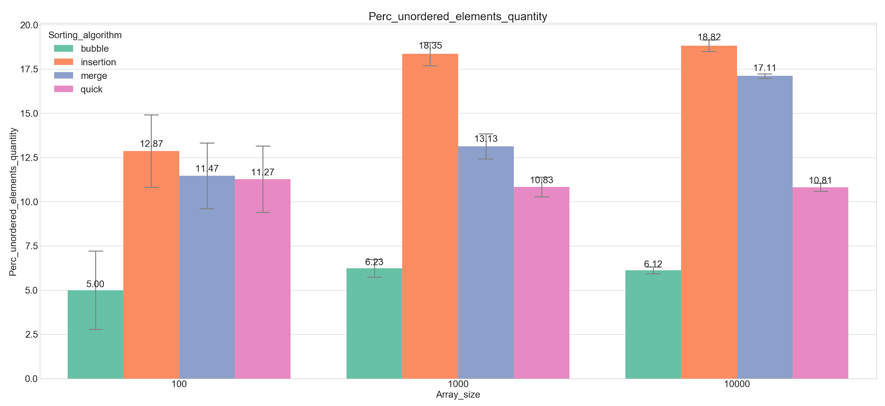
\includegraphics[scale=1.15]{figures/Barplot_Estatisticas_por_Algoritmo_Prob_0_02.png}}
    \textsf{\caption[Data for \textit{probability of failure} of 2\%.]{Data for \textit{probability of failure} of 2\%.\label{fig-barplot-pof-002}}}
 \end{figure}

 \begin{figure}[H]
    \centering
    \frame{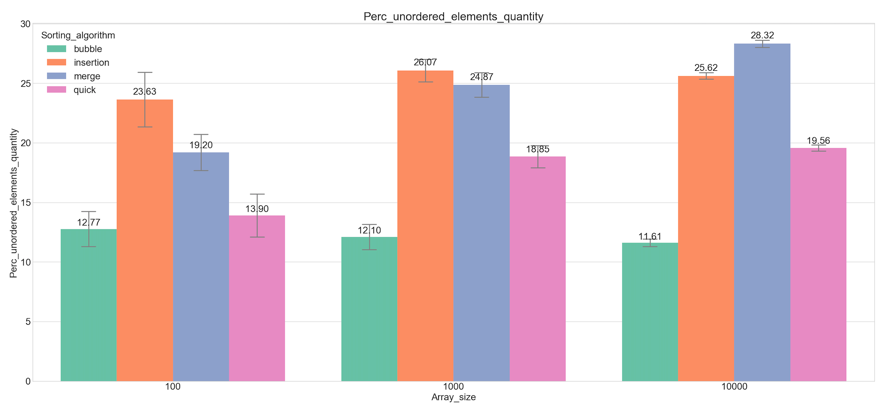
\includegraphics[scale=1.15]{figures/Barplot_Estatisticas_por_Algoritmo_Prob_0_05.png}}
    \textsf{\caption[Data for \textit{probability of failure} of 5\%.]{Data for \textit{probability of failure} of 5\%.\label{fig-barplot-pof-005}}}
\end{figure}

Considering the data in the graphs, we can conclude that Bubblesort generates lower mean value for variable \%UEQ for all defined combinations (\textit{probability of failure} X \textit{array size} X \textit{sorting algorithm}). These data demonstrate that Bubblesort was the less affected algorithm by the memory faults simulated in this experiment. We believe that this fact happened because of the operation of the algorithm itself, where all elements order are verified each iteration, causing an element incorrectly positioned in an iteration (because of a memory fault) can have its location corrected in an upcoming iteration.

Related to Bubblesort yet, we could identify that despite different sizes of input arrays (100, 1000, and 10000), there was not a significant impact on the mean value obtained for \%UEQ variable, proving what we verify with ANOVA when doing hypothesis 3 testing for this algorithm.